\documentclass[document.tex]{subfiles} 
\begin{document}

\clearpage\section{Использование библиотеки для синтеза устройств}
В разделе представлены способы использования библиотеки для синтеза типов
устройств.

Общий принцип синтеза устройств с использованием программной библиотеки --
создание экземпляра класса соответствующего устройства с заполнением
количества входных и выходных типов сигналов, перечисленных в классе устройства
обязательными к заполнению.
\subsection{Логические вентили}
Логический вентиль -- базовый элемент цифровой схемы, выполняющий элементарную
логическую операцию, преобразуя таким образом множество входных логических
сигналов в выходной логический сигнал. Логика работы вентиля основана на битовых
операциях с входными цифровыми сигналами в качестве операндов. При создании
цифровой схемы вентили соединяют между собой, при этом выход используемого
вентиля должен быть подключен к одному или к нескольким входам других
вентилей~\cite{wikigates}.

Вся кодовая база логических вентилей находится в пакете devices.simple и
наследуется от абстрактного класса DeviceSimple.

В разрабатываемой библиотеке на настоящий момент присутствует техническое
ограничение, не позволяющее задавать базис и ограничение на количество разрядов
логических вентилей в составных устройствах. Это ограничение связано с
использованием библиотеки символьной алгебры, не предоставляющей функционал
ленивых логических вычислений. Все логические выражения символьной алгебры в
составных устройствах раскрываются и упрощаются автоматически~\cite{sympydoc}.

\clearpage
\subsubsection{Логический вентиль НЕ (инвертор)}
Логический вентиль НЕ (инвертор) с
возможностью поразрядной инверсии можно описать следующим образом:
\begin{equation}
\label{eq:not}
\forall x: O_x = \overline{I_x}
\end{equation}

В выражении~\ref{eq:not}:
\begin{itemize}[noitemsep]
  \item $x$ -- индекс входного разряда;
  \item $I$ -- набор входных разрядов;
  \item $O$ -- набор выходных разрядов.
\end{itemize}

Описание логического вентиля НЕ в разрабатываемой библиотеке представлено в
листинге~\ref{lst:not}.

\begin{listing}[ht]
\begin{minted}[linenos=true]{python}
class DeviceNot(DeviceSimple):
    """Logic NOT gate"""
    logic_function = Not
    constraints = {
        'data_signals': {
            'min': 1,
            'max': 10
        },
        'output_signals': {
            'min': 1,
            'max': 10
        }
    }

    @property
    def functions(self):
        return [self.logic_function(signal) for signal in self.data_signals]
\end{minted}
\caption{Программное описание класса логического вентиля НЕ}
\label{lst:not}
\end{listing}

\clearpage
В листинге~\ref{lst:notgen} представлен код для программного синтеза
устройства инвертора с 3 входными разрядами данных (data\_signals='d:3') и 3
выходными разрядами (output\_signals='o:3').

\begin{listing}[ht]
\begin{minted}{pycon}
>>> from circuitry.devices.simple import DeviceNot
>>> pprint(  
...     DeviceNot(data_signals='d:3', output_signals='o:3')
... )
{'data_signals': (d0, d1, d2),
 'output_signals': (o0, o1, o2),
 'truth_table': [([0, 0, 0], [1, 1, 1]),
                 ([1, 0, 0], [0, 1, 1]),
                 ([0, 1, 0], [1, 0, 1]),
                 ([1, 1, 0], [0, 0, 1]),
                 ([0, 0, 1], [1, 1, 0]),
                 ([1, 0, 1], [0, 1, 0]),
                 ([0, 1, 1], [1, 0, 0]),
                 ([1, 1, 1], [0, 0, 0])]}
\end{minted}
\caption{Программный синтез логического вентиля НЕ}
\label{lst:notgen}
\end{listing}

На рисунке~\ref{fig:devicenot} представлено условно-графическое обозначение
синтезированного вентиля НЕ.

\begin{figure}[here]
\centering
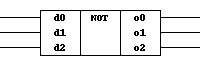
\includegraphics{devices_not_sym}
\caption{Условно-графическое обозначение вентиля НЕ}
\label{fig:devicenot}
\end{figure}

\clearpage
\subsubsection{Логический вентиль И (конъюнкция)}
Логический вентиль И (логическое умножение, конъюнкция) описывается следующим
образом:
\begin{equation}
\label{eq:and}
O_0 = I_0 \wedge I_2 \wedge \ldots \wedge I_{n - 1}
\end{equation}

В выражении~\ref{eq:and}:
\begin{itemize}[noitemsep]
  \item $n$ -- количество входных разрядов;
  \item $I$ -- набор входных разрядов;
  \item $O_0$ -- выходной разряд.
\end{itemize}

Описание логического вентиля И в разрабатываемой библиотеке представлено в
листинге~\ref{lst:and}.

\begin{listing}[ht]
\begin{minted}[linenos=true]{python}
class DeviceAnd(DeviceSimple):
    """Logic AND gate"""
    logic_function = And
    constraints = {
        'data_signals': {
            'min': 2,
            'max': 10
        },
        'output_signals': {
            'min': 1,
            'max': 1
        }
    }
\end{minted}
\caption{Программное описание класса логического вентиля И}
\label{lst:and}
\end{listing}

\clearpage
В листинге~\ref{lst:andgen} представлен код для программного синтеза
устройства логического умножения с 2 входными разрядами данных
(data\_signals='d:2') и 1 прямым выходным разрядом (output\_signals='o:1').

\begin{listing}[ht]
\begin{minted}{pycon}
>>> from circuitry.devices.simple import DeviceAnd
>>> pprint(                                                                                
...     DeviceAnd(data_signals='d:2', output_signals='o:1',
...               output_signals_subs=dict(o0=1))
... )
{'data_signals': (d0, d1),
 'output_signals': (o0,),
 'output_signals_function': o0,
 'output_signals_subs': {'o0': 1},
 'output_signals_truth_table': [1],
 'truth_table': [([0, 0], [0]), ([1, 0], [0]), ([0, 1], [0]), ([1, 1], [1])]}
\end{minted}
\caption{Программный синтез логического вентиля И}
\label{lst:andgen}
\end{listing}

На рисунке~\ref{fig:deviceand} представлено условно-графическое обозначение
синтезированного вентиля И.

\begin{figure}[here]
\centering
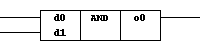
\includegraphics{devices_and_sym}
\caption{Условно-графическое обозначение вентиля И}
\label{fig:deviceand}
\end{figure}

\clearpage
\subsubsection{Логический вентиль ИЛИ (дизъюнкция)}
Логический вентиль ИЛИ (логическое сложение, дизъюнкция) описывается следующим
образом:
\begin{equation}
\label{eq:or}
O_0 = I_0 \vee I_2 \vee \ldots \vee I_{n - 1}
\end{equation}

В выражении~\ref{eq:or}:
\begin{itemize}[noitemsep]
  \item $n$ -- количество входных разрядов;
  \item $I$ -- набор входных разрядов;
  \item $O_0$ -- выходной разряд.
\end{itemize}

Описание логического вентиля ИЛИ в разрабатываемой библиотеке представлено в
листинге~\ref{lst:or}.

\begin{listing}[ht]
\begin{minted}[linenos=true]{python}
class DeviceOr(DeviceSimple):
    """Logic OR gate"""
    logic_function = Or
    constraints = {
        'data_signals': {
            'min': 2,
            'max': 10
        },
        'output_signals': {
            'min': 1,
            'max': 1
        }
    }
\end{minted}
\caption{Программное описание класса логического вентиля ИЛИ}
\label{lst:or}
\end{listing}

\clearpage
В листинге~\ref{lst:orgen} представлен код для программного синтеза
устройства логического сложения с 3 входными разрядами данных
(data\_signals='d:3') и 1 прямым выходным разрядом (output\_signals='o:1').

\begin{listing}[ht]
\begin{minted}{pycon}
>>> from circuitry.devices.simple import DeviceOr 
>>> pprint(                                                
...     DeviceOr(data_signals='d:3', output_signals='o:1',
...               output_signals_subs=dict(o0=1))         
... )
{'data_signals': (d0, d1, d2),
 'output_signals': (o0,),
 'output_signals_function': o0,
 'output_signals_subs': {'o0': 1},
 'output_signals_truth_table': [1],
 'truth_table': [([0, 0, 0], [0]),
                 ([1, 0, 0], [1]),
                 ([0, 1, 0], [1]),
                 ([1, 1, 0], [1]),
                 ([0, 0, 1], [1]),
                 ([1, 0, 1], [1]),
                 ([0, 1, 1], [1]),
                 ([1, 1, 1], [1])]}
\end{minted}
\caption{Программный синтез логического вентиля ИЛИ}
\label{lst:orgen}
\end{listing}

На рисунке~\ref{fig:deviceor} представлено условно-графическое обозначение
синтезированного вентиля ИЛИ.

\begin{figure}[here]
\centering
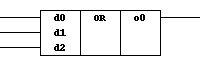
\includegraphics{devices_or_sym}
\caption{Условно-графическое обозначение вентиля ИЛИ}
\label{fig:deviceor}
\end{figure}

\end{document}